\documentclass[border=4pt]{standalone}
% Preámbulo común de las figuras. Cada figura es un documento standalone
% que se compila a SVG con scripts/build_figures.sh
\usepackage[utf8]{inputenc}
\usepackage{amsmath}
\usepackage{tikz}
\usepackage[american, siunitx]{circuitikz}
\usetikzlibrary{arrows.meta,calc,decorations.pathmorphing,patterns}
\tikzset{
  >={Stealth[length=2.2mm]},
  eje/.style={->, thin},
  hilo/.style={thick},
}
% Paleta común: tonos medios legibles sobre fondo claro
\definecolor{azul}{RGB}{31,94,168}
\definecolor{rojo}{RGB}{192,57,43}
\definecolor{verde}{RGB}{39,128,73}
\definecolor{naranja}{RGB}{211,120,30}
\definecolor{morado}{RGB}{125,60,152}

\begin{document}
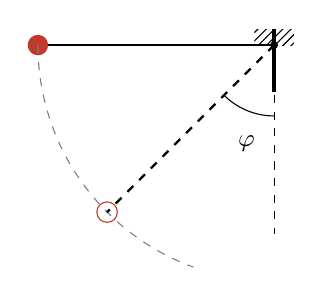
\begin{tikzpicture}[scale=1.0]
  \fill[pattern=north east lines] (3.0,0.2) rectangle (3.5,-0.0);
  \draw[very thick] (3.25,0.2) -- (3.25,-0.6);
  \fill (3.25,0) circle (1.4pt);
  \draw[hilo] (3.25,0) -- (0.25,0);
  \fill[rojo] (0.25,0) circle (0.13);
  \draw[dashed, gray] (0.25,0) arc[start angle=180, end angle=250, radius=3.0];
  \draw[hilo, dashed] (3.25,0) -- ({3.25 + 3.0*cos(225)},{3.0*sin(225)});
  \draw[rojo] ({3.25 + 3.0*cos(225)},{3.0*sin(225)}) circle (0.13);
  \draw[dashed] (3.25,0) -- (3.25,-2.4);
  \draw (3.25,-0.9) arc[start angle=270, end angle=225, radius=0.9];
  \node[font=\small] at (2.9,-1.25) {$\varphi$};
\end{tikzpicture}
\end{document}
